%\title{LaTeX Portrait Poster Template}
%%%%%%%%%%%%%%%%%%%%%%%%%%%%%%%%%%%%%%%%%
%
% Henriques lab poster template 
% Version 1.0 (13/04/2019)
% Originally based on:
%
% a0poster Portrait Poster
% LaTeX Template
% Version 1.0 (22/06/13)
%
% The a0poster class was created by:
% Gerlinde Kettl and Matthias Weiser (tex@kettl.de)
% 
% This template has been downloaded from:
% http://www.LaTeXTemplates.com
%
% License:
% CC BY-NC-SA 3.0 (http://creativecommons.org/licenses/by-nc-sa/3.0/)
%
%%%%%%%%%%%%%%%%%%%%%%%%%%%%%%%%%%%%%%%%%

%----------------------------------------------------------------------------------------
%	PACKAGES AND OTHER DOCUMENT CONFIGURATIONS
%----------------------------------------------------------------------------------------

\documentclass[a0,portrait]{a0poster}

\usepackage{multicol} % This is so we can have multiple columns of text side-by-side
\columnsep=50pt % This is the amount of white space between the columns in the poster
\columnseprule=0pt % This is the thickness of the black line between the columns in the poster

\usepackage[svgnames]{xcolor} % Specify colors by their 'svgnames', for a full list of all colors available see here: http://www.latextemplates.com/svgnames-colors

\usepackage{times} % Use the times font
%\usepackage{palatino} % Uncomment to use the Palatino font

\graphicspath{{figures/}} % Location of the graphics files
\usepackage{booktabs} % Top and bottom rules for table
\usepackage[font=small,labelfont=bf]{caption} % Required for specifying captions to tables and figures
\usepackage{amsfonts, amsmath, amsthm, amssymb} % For math fonts, symbols and environments
\usepackage{wrapfig} % Allows wrapping text around tables and figures
\usepackage[labelformat=empty]{caption}
\usepackage{fontawesome}
\usepackage{listings}% code 
\begin{document}

%----------------------------------------------------------------------------------------
%	POSTER HEADER 
%----------------------------------------------------------------------------------------

% The header is divided into two boxes:
% The first is 75% wide and houses the title, subtitle, names, university/organization and contact information
% The second is 25% wide and houses a logo for your university/organization or a photo of you
% The widths of these boxes can be easily edited to accommodate your content as you see fit


\begin{minipage}[b]{0.75\linewidth}
\VeryHuge \color{NavyBlue} \textbf{Transfer Operator Methods - Transport 2d Electron Gases}
\color{Black}\\[0.4cm] 
\Large \textbf{Mingdong He}\\
\Large \textbf{Supervisor: Martin Richter}\\
\large \textbf{School of Mathematical Sciences, University of Nottingham}\\ 
\large \textbf{\Letter \space smymh1@nottingham.ac.uk}\\
\large \textbf{\faGithub \space 
https://github.com/Homingdung/2deg\_billiard\_matlab}
\end{minipage}
%
%\begin{minipage}[b]{0.25\linewidth}
%\begin{center}
%
\includegraphics[width=20cm]{logo.png}\\ 
%\end{center}
%\end{minipage}

%\vspace{.2cm} % A bit of extra whitespace between the header and poster content

%----------------------------------------------------------------------------------------

\begin{multicols}{3} % This is how many columns your poster will be broken into, a portrait poster is generally split into 2 columns

%----------------------------------------------------------------------------------------
%	Introduction
%----------------------------------------------------------------------------------------
\section*{Introduction}
\noindent
This project is based on an experiment \cite{richterklassischer} as shown in \textbf{FIG. \ref{fig:composite}}: the electrons \cite{boggild1999magnetic} are emitted to a triangular cavity through a narrow hole with a magnetic field and the electrons will collide with the walls of the cavity as billiards. As the electrons leaving will give rise to electric resistance, the graph of how resistance changes with magnetic field indicates a dual peak phenomenon, which seems to match the reflections in cavity. Due to the complexity of the behavior of the electrons in the cavity, it seems that quantum mechanics, randomness, uncertainty, and PDE etc. would be considered to account for this dual peak phenomenon. In order to study this problem from a computational simplicity view, we simplify the problem as 2d electron gases (2DEG) and proposed a 2-dimensional model based on Birkhoff coordinate and transfer operator to reproduce the experiment by using analytical ODE solution and numerical simulations for the dynamics of the billiards.

\begin{center}\vspace{1cm}
    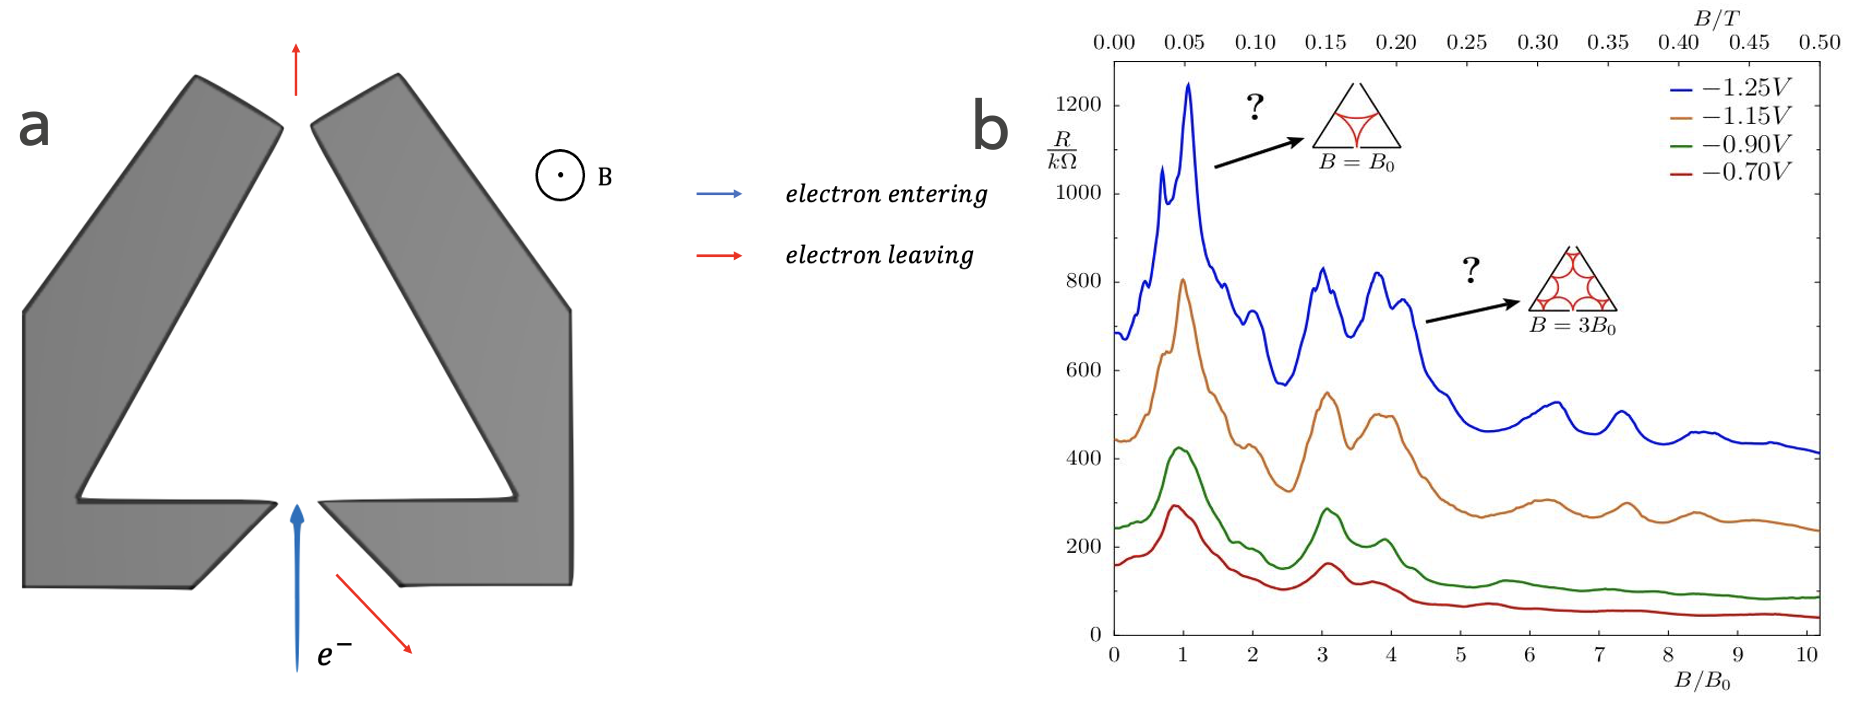
\includegraphics[width=0.8\linewidth]{composite.png}
    \captionof{figure}{\textbf{FIG. 1.}} \textbf{a)}The electrons emitted through a narrow hole with an initial distribution. Point reflections happened due to the collision with the walls of cavity. \textbf{b)} The electrons leaving will generate resistance.
    \label{fig:composite}
%\captionof{figure}{\textbf{NanoJ framework.} Currently NanoJ consists of 5 modules dedicated to super-resolution imaging and analysis.}
\end{center}%\vspace{1cm}

%----------------------------------------------------------------------------------------
%	Methodology
%----------------------------------------------------------------------------------------
\section*{Methodology}

\noindent
We simplify the dynamics of the 2DEG with unit mass in a closed hard wall regular triangle cavity with length 1 for each side, which could be described as an ODE system shown in (1) and a billiard is a Hamiltonian system with potential $V=0$:

\begin{equation}
\begin{aligned}
& \frac{dx}{dt}=v_x\\
\\
& \frac{dy}{dt}=v_y\\
\\
& \frac{d v_x}{dt}=2\sqrt{2}Bv_y-\frac{\partial V}{\partial x}(x,y)=2\sqrt{2}Bv_y\\
\\
& \frac{d v_y}{dt}=-2\sqrt{2}Bv_x-\frac{\partial V}{\partial y}(x,y)=-2\sqrt{2}Bv_x\\
\end{aligned}
\end{equation}

The conservation of energy makes the 2-dimensional problem sufficient to consider only 1 parameter for velocity, $p$, the projected momentum on the boundary. We also rescale the parameters and get the value of velocity as $\sqrt{2}$. Thus, the emitting electron could be considered as one from the position $(x_0,y_0)$ with initial velocity $v_0=(\sqrt{2}p,\sqrt{2}\sqrt{1-p^2})$, where $p \in [-1,1]$

Thus, the analytical solution results in orbit due to the magnetic field:
%analytical solution---------------

\begin{equation}
\begin{aligned}
& R=R(B)=\frac{|v_0|}{2\sqrt{2}|B|}\\
& \omega=-2\sqrt{2}B\\
& X_{centre}=(x_c,y_c)=(x_0-\frac{v_{y_0}}{\omega},y_0+\frac{v_{x_0}}{\omega})\\
& \phi=arctan(\frac{y_0-y_c}{x_0-x_c})\\
& (x(t),y(t))=(x_c+Rcos(\omega t+\phi), y_c+Rsin(\omega t+\phi))\\
\end{aligned}
\end{equation}

%nomenclature------------------------
\begin{tabular}{cccc}
\toprule
$(x,y)$ & position & $p$ & projected momentum  \\
$(x_0,y_0)$ & initial position & $R$ & radius of orbit \\
$(v_x,v_y)$ & velocity & $\omega$ & angular velocity \\
$(v_{x_0},v_{y_0})$ & initial velocity & $\phi$ &phase \\
$V$ & potential & $B$ & magnetic field \\
$(x_c,y_c)$ & orbit centre &&\\
\bottomrule
\end{tabular}
\begin{center}
    \textbf{Table 1}: Nomenclature for the equations above
\end{center}

%----------------------------------------------------------------------------------------
%	Birkhoff coordinate
%----------------------------------------------------------------------------------------

Birkhoff coordinate, also known as boundary coordinate, which can be used to define a natural Poincaré section for billiard flow \cite{cvitanovic2020chaos}, specifies the collision point, with which could also be displayed on a phase-space with $(s,p)$, where $s$ is the position along the boundary and $p$ is the projected momentum on the boundary. \textbf{FIG. \ref{fig:composite2}} shows how the reflection occurs. We use a combined coordinate system (Cartesian and Polar) to derive the Birkhoff coordinate $(s,p)$ as shown in \textbf{FIG. \ref{fig:composite2}}.

\begin{center}\vspace{1cm}
    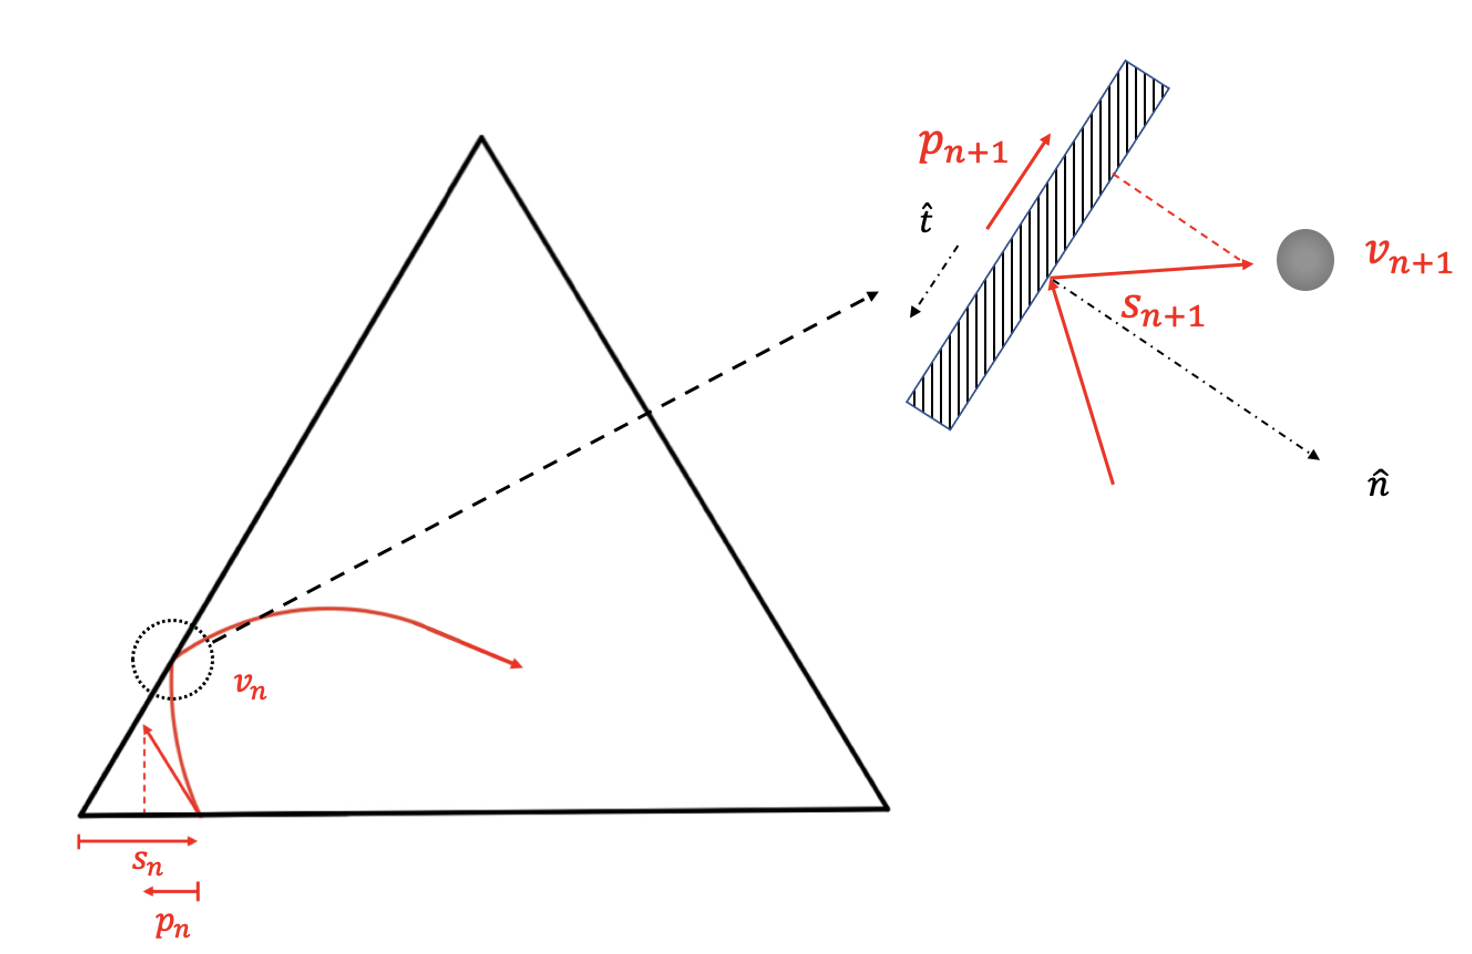
\includegraphics[width=0.5\linewidth]{projection2.png}
    \captionof{figure}{\textbf{FIG. 2.} Trajectories specified by Birkhoff coordinates. The 2DEG collides with the wall and will be reflected, where $\hat{t}$ is the unit tangential vector and $\hat{n}$ is the unit normal vector.}
    \label{fig:projection2}
\end{center}%\vspace{1cm}

\begin{center}\vspace{1cm}
    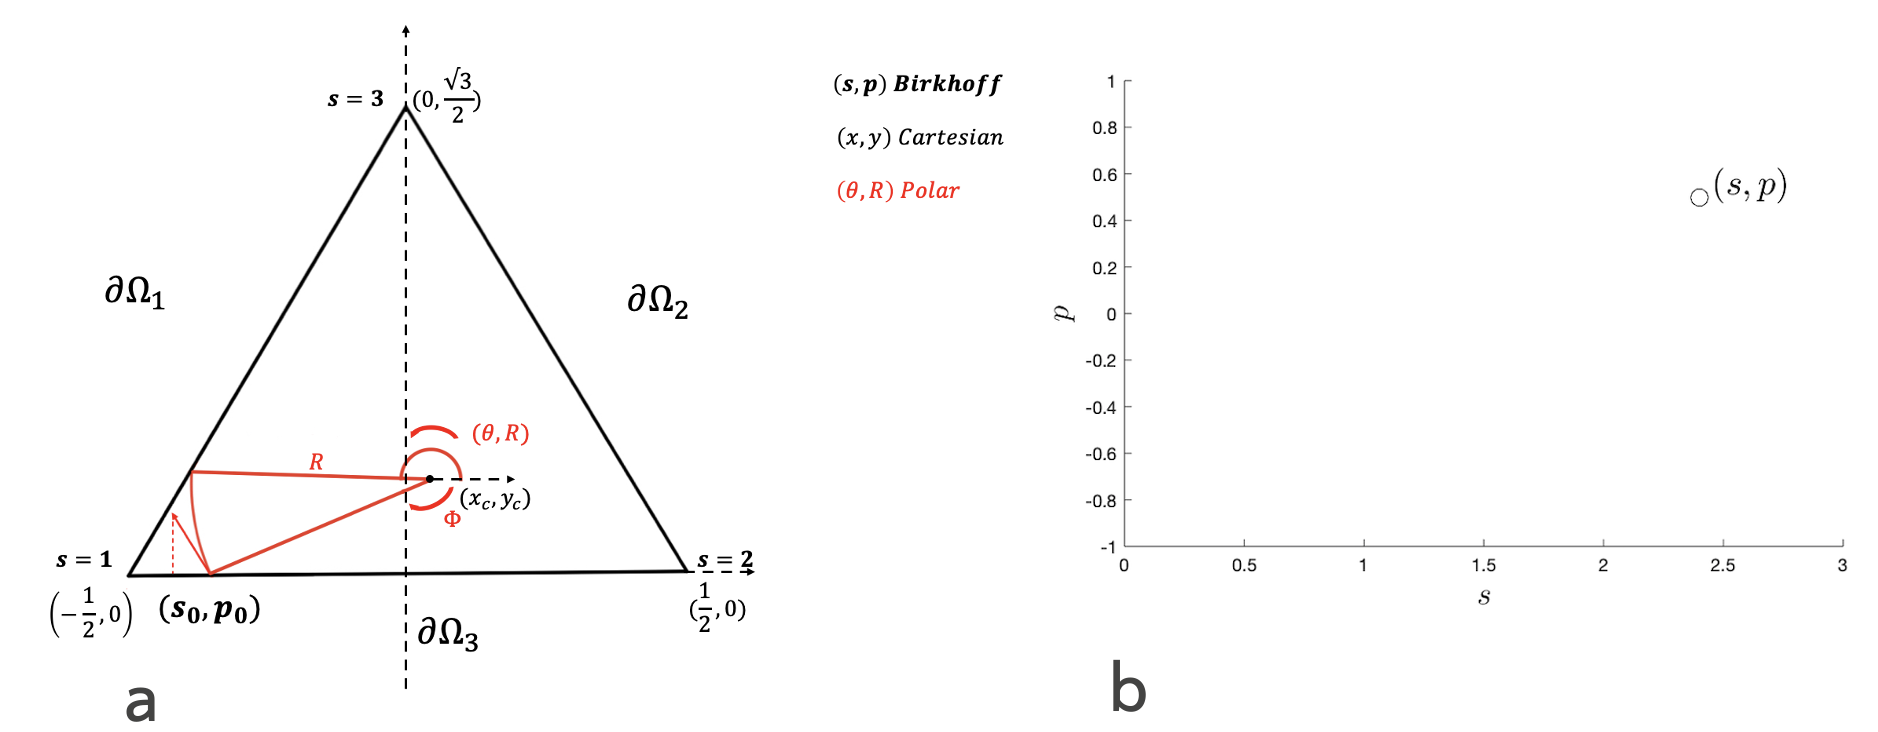
\includegraphics[width=0.8\linewidth]{composite2.png}
    \captionof{figure}{\textbf{FIG. 3.} \textbf{a)} The 2DEG is about to collide with the wall $\partial \Omega_1$, $\partial \Omega_2$, $\partial \Omega_3$} \textbf{b)} Birkhoff phace-space.
    \label{fig:composite2}
\end{center}%\vspace{1cm}


\section*{Numerical solution and simulation}
%----------------------------------------------------------------------------------------
%	numerical recipes
%----------------------------------------------------------------------------------------

\noindent
We define the Poincaré map $M_B$ for the billiard from the $n$th collision to the $(n+1)$st collision to describe the dynamics, which could be found numerically by the following recipes:
\begin{itemize}
    \item $M_B: (s_n, p_n) \to (s_{n+1},p_{n+1}), n=0, 1, 2...$, $(s,p): (0, 3) \times [-1, 1]$
    \item Set $s_0 \in (0, 1),p_0 \in [-1,1], B>0$
    \item Calculate the potential collision points on each wall after the first mapping\\
$\partial \Omega_1$:
\begin{equation}
\begin{aligned}
& \theta=\frac{1}{2R}sin^{-1}(\frac{\sqrt{3}}{2}x_c+\frac{\sqrt{3}}{2}-y_c)+\frac{\pi}{3}\\
\\
& s=3-\frac{2}{\sqrt{3}}(y_c+Rsin(\theta))\\
\\
& p=\frac{R\omega}{\sqrt{2}}sin(\theta-\frac{\pi}{3})
\end{aligned}
\end{equation}
$\partial \Omega_2$:
\begin{equation}
\begin{aligned}
& \theta=\frac{1}{2R}sin^{-1}(-\frac{\sqrt{3}}{2}x_c+\frac{\sqrt{3}}{2}-y_c)-\frac{\pi}{3}\\
& s=1+\frac{2}{\sqrt{3}}(y_c+Rsin(\theta))\\
& p=\frac{R\omega}{\sqrt{2}}sin(\theta+\frac{\pi}{3})
\end{aligned}
\end{equation}

$\partial \Omega_3$:
\begin{equation}
\begin{aligned}
& s=s_0+2Rcos(\pi-\phi)\\
& p=p_0
\end{aligned}
\end{equation}
    \item Select the correct point as prediction for $(s_1,p_1)$ by algorithm \textbf{FIG.\ref{flowchat}}, where the $d_1$ $d_2$ $d_3$ is the distance from the centre to the  chord formed by the adjacent reflection points $(s_0,p_0)$ and $(s_1,p_1)$ on each wall, and $R$ is the radius of the orbit.

\begin{center}\vspace{1cm}
    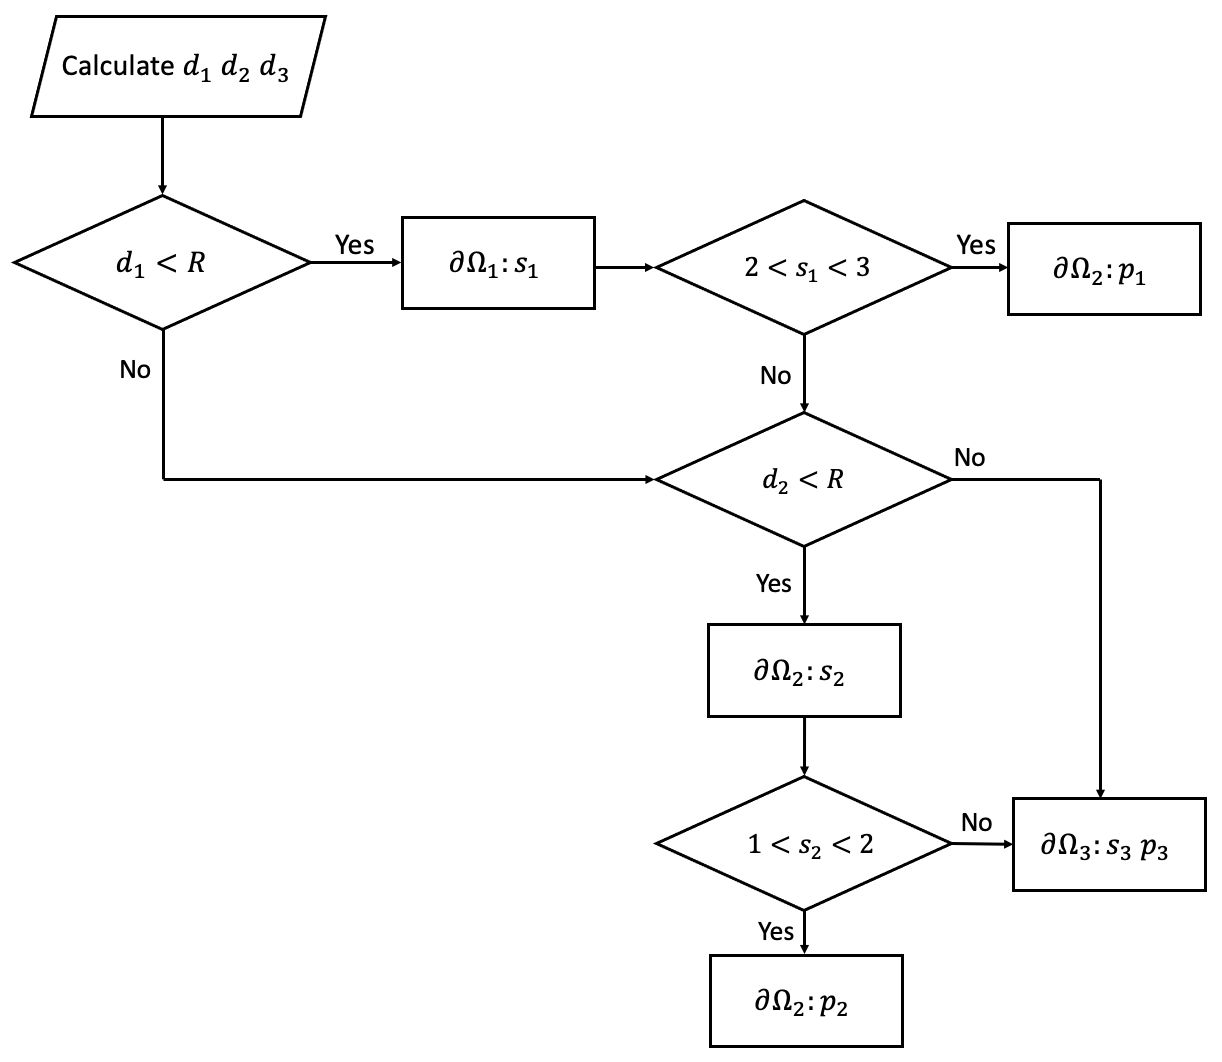
\includegraphics[width=0.5\linewidth]{flowchat.png}
    \captionof{figure}{\textbf{FIG. 4.}Algorithm to select the correct collision point}
    \label{flowchat}
\end{center}%\vspace{1cm}
\item Define an initial density function $\rho^{\delta}_0(s,p)$ and the transfer operator $T^{\alpha}_{\rho}, \alpha=3,9$
\begin{equation}
\rho_a^{\delta}(s,p) =\left\{
	\begin{aligned}
	&0 \quad |s-\frac{1}{2}|>\frac{\delta}{2}\\
	&cos^{2n}(\frac{\pi}{\delta}(s-\frac{1}{2})) \quad |s-\frac{1}{2}|\leq\frac{\delta}{2}\\
	\end{aligned}
	\right
.
\end{equation}
\begin{equation}
\rho_0^{\delta} (s,p)= \rho_a^{\delta}(s,p) \ cos^{2m}(\frac{\pi}{2}p)
\end{equation}\\
\begin{equation}
\begin{aligned}
& T^3\rho=\rho \ \circ M^{-1} \circ M^{-1} \circ M^{-1}\\
& T^9\rho=\rho \ \circ \underbrace{M^{-1} \circ ... \circ M^{-1}}_{9}
\end{aligned}
\end{equation}
\end{itemize}

Assuming that the 2DEG will not collide the walls less than 3 reflections and 9 reflections, respectively, we integrate the transfer operator to get the amount of 2DEG leaving the hole from the $\partial \Omega_3$:

\begin{equation}
r(B)=\int T^{\alpha}_{\rho} dS=\int_{-1}^{1}\int_{1/2-\delta/2}^{1/2+\delta/2} T^{\alpha}_{\rho} dsd\rho=\Delta s \Delta \rho \sum_{ij} \rho_{\alpha}(s_i,p_j)
\end{equation}
%----------------------------------------------------------------------------------------
%	MATLAB simulation
%----------------------------------------------------------------------------------------

MATLAB simulation could give us the boundary map based on Birkhoff phase-space in \textbf{FIG. \ref{compositeB}} for $B=0.5, 1.1, 1.2$, together with the initial density function with $\delta=0.05, n=2, m=3$. These points are generated by our Poincaré map

\begin{equation}
M_B: \{(s_n,p_n)\}=\{M^n_B(s_0,p_0)\}, n=0,1,2...   
\end{equation}

Fixed points can be seen in the phase-space within the triangles and when $s=0.5$, we could find orbits, which match the reflections in the cavity. The shape of boundary map changes from an inverted triangle to a normal triangle as B changes from 0.4 to 1.2. It is noticeable that the fixed point shows stable at the beginning, then unstable and finally becomes stable again when the magnetic field values $B$ increases, which is known as Bifurcation. 

\begin{center}\vspace{1cm}
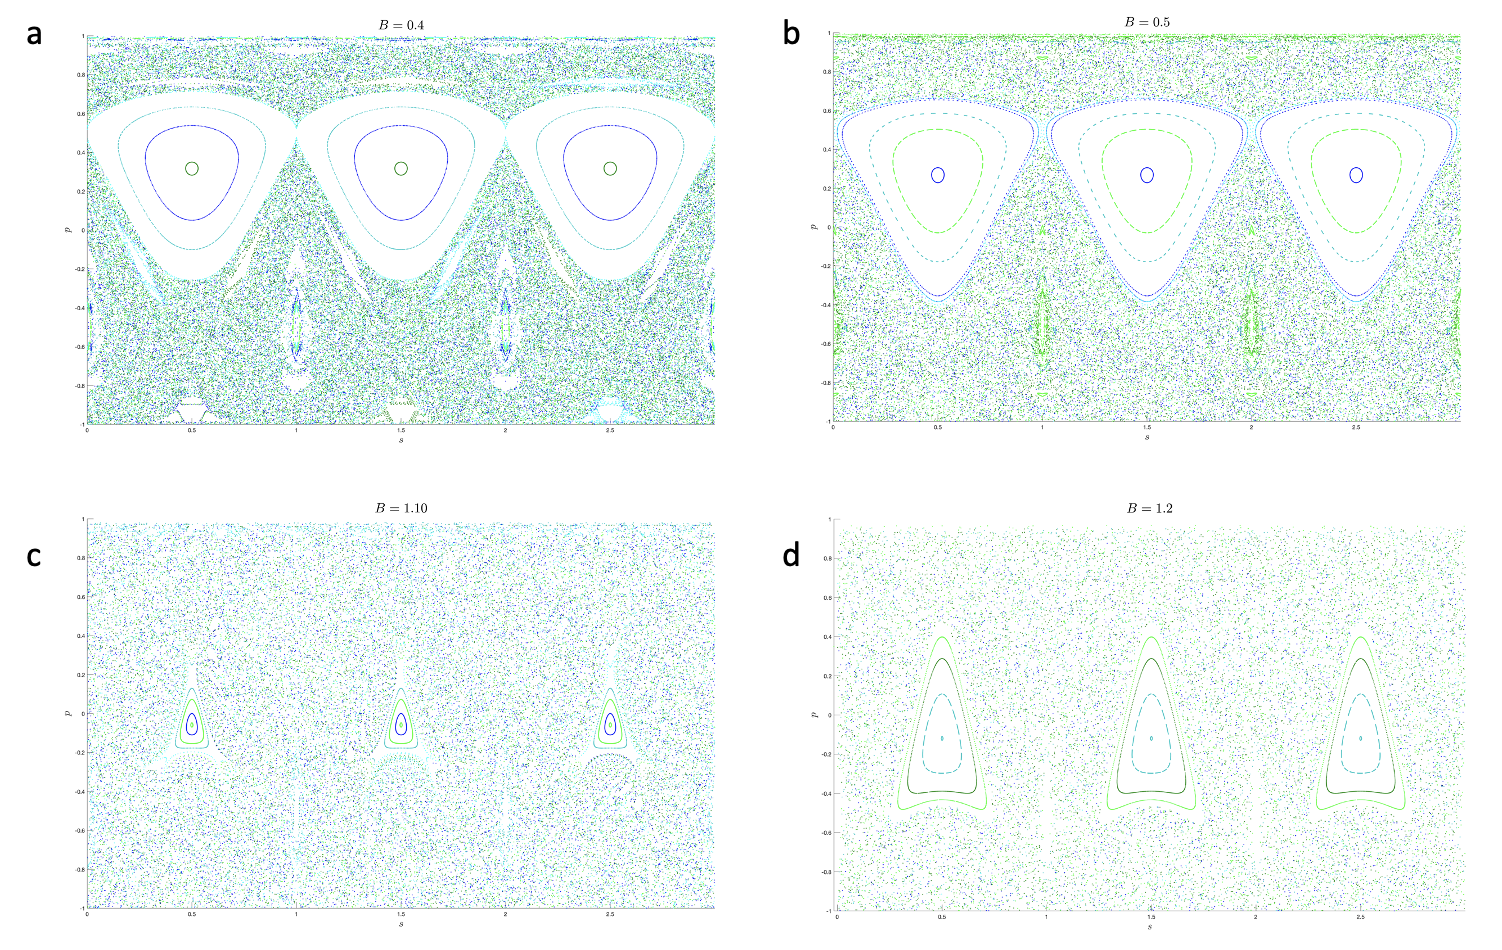
\includegraphics[width=0.85\linewidth]{compositeB.png}
\captionof{figure}{\textbf{FIG. 5.} Boundary map for \textbf{a)} $B=0.4$ \textbf{b)} $B=0.5$ \textbf{c)} $B=1.1$ \textbf{d)} $B=1.2$ Bifurcation occurs when increasing the $B$ from 0.4 to 1.2 }
\label{compositeB}
\end{center}%\vspace{1cm}

In \textbf{FIG. \ref{compositerho} d)}, it is obvious that the numerical simulation of our model also shows dual peak when $B=1.0$.
\begin{center}\vspace{1cm}
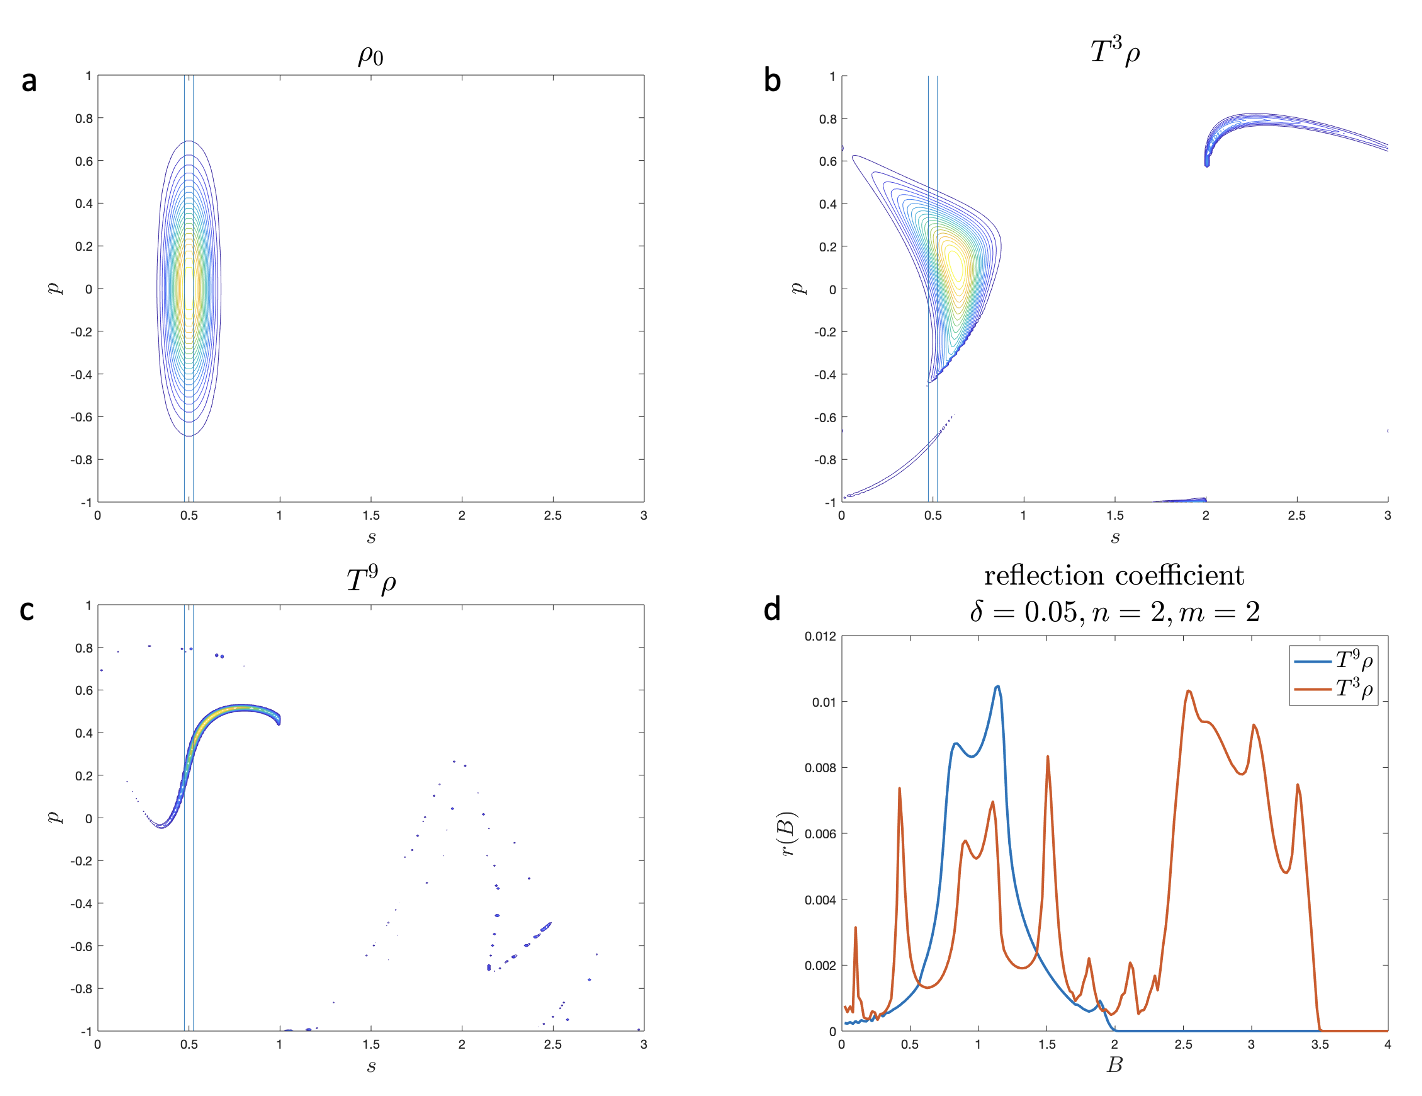
\includegraphics[width=0.85\linewidth]{compositerho.png}
\captionof{figure}{\textbf{FIG. 6.} Boundary map for initial density function and transfer operators. The two vertical lines control the emitting hole. \textbf{a)} initial density function \textbf{b)} transfer operator for 3 reflections \textbf{c)} transfer operator for 9 reflections \textbf{d)} resistance vs magnetic field for different transfer operators. It also indicates that the dual peaks occurs in cavity based on the numerical simulation of our model compared with the \textbf{FIG. 1. b)}.}
\label{compositerho}
\end{center}%\vspace{1cm}


% %----------------------------------------------------------------------------------------
% %	CONCLUSIONS
% %----------------------------------------------------------------------------------------
\section*{Conclusion}
\begin{itemize}
    \item We use our derived transfer operator methods to investigate the dynamics of 2DEG displayed by boundary map.
    \item Numerical simulation indicates a consistence with the experimental result for the dual peak phenomenon by a computationally easy approach without using quantum mechanics, randomness, uncertainty and PDE etc.
    \item Although the assumption that 2DEG will not collide the walls less than 3 reflections and 9 reflections makes the model computationally easy, it is not true. For instance, the 2DEG could escape the cavity by just one reflections.
    \item Further study could focus on more complete cases for the dynamics of billiards and the bifurcation of boundary map is also worth studying.
\end{itemize}

%----------------------------------------------------------------------------------------
%	References
%----------------------------------------------------------------------------------------

\small
\nocite{*} % Print all references regardless of whether they were cited in the poster or not
\bibliographystyle{plain} % Plain referencing style
\bibliography{sample} % Use the example bibliography file sample.bib

%----------------------------------------------------------------------------------------
%	Funding
%----------------------------------------------------------------------------------------
\section*{Funded by}
\begin{center}\vspace{0cm}

\includegraphics[width=0.95\linewidth]{logo.png}
\end{center}%\vspace{1cm}

\section*{Acknowledgement}
This research internship is supported by the School of Mathematical Sciences, University of Nottingham. I would like to say special thank you to my supervisor Martin Richter for his nice support and guidance, and others who have supported me throughout this internship.


%----------------------------------------------------------------------------------------

\end{multicols}
\end{document}